\chapter{Straight Line Programs}

In this chapter we introduce the language of \emph{straight line} programs which can be considered as a smallest
non-trivial subset of \lama. In this subset all programs are executed sequentially statement by statement with
no branching. Thus, any program either comes to an end or stops due to an error, but cannot loop forever. We
use this simple language to showcase all the ingredients of our approach to language description: abstract and
concrete syntax specification, denotational and operational semantics, etc. We also introduce some components of
the compiler we will be working on: source-level interpreter, stack machine compiler and interpreter, and
\texttt{x86} code generator.

\begin{figure}[t]
  \centering
  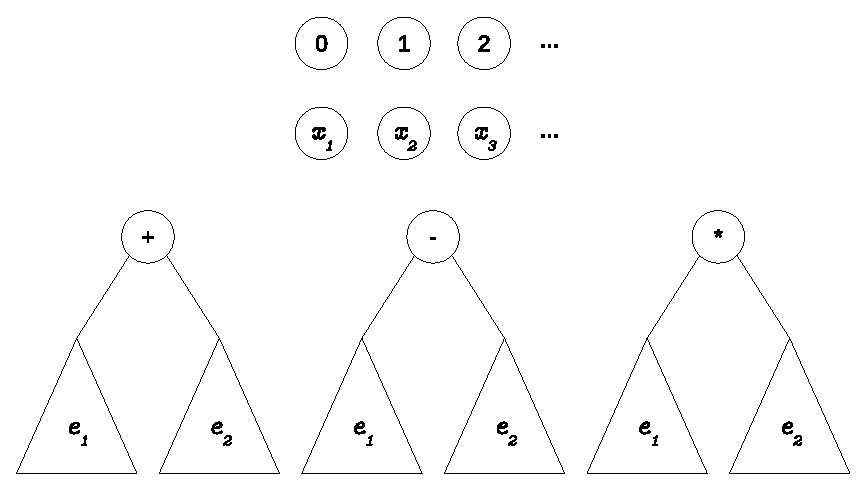
\includegraphics[scale=0.7]{images/02-01.eps}
  \caption{Abstract Syntax for Expressions}
  \label{expression-syntax}
\end{figure}

\section{Expressions}


Syntactically, our language encorporates two \emph{syntactic categories}: expressions and statements. We start from describing
so-called \emph{abstract syntax} for the expression category. We consider a countable set of \emph{variables}

\[
\mathscr{X}=\{x_1,\,x_2,\,\dots\}
\]

and a set of \emph{binary operators}

\[
\otimes= \{+,\, -,\, \times,\, /,\, \%,\, <,\, \le,\, >,\, \ge,\, =,\,\ne,\, \vee,\, \wedge\}
\]

which contains all thirteen built-in \lama operators. Then, the category of expressions $\mathscr{E}$ can be defined by
the following recursive scheme:

\[
\begin{array}{rcl}
  \mathscr{E} & = & \mathscr{X} \\
              &   & \mathbb{N} \\
              &   & \mathscr{E}\otimes\mathscr{E}
\end{array}
\]

This scheme defines a countable set of \emph{labeled ordered trees} of finite height: each node of such a tree is labeled, and for any node the order
of its immediate subtrees is essential. The simplest trees of this form are just leaves labeled with either variables or natural numbers; we simply
write $\mathscr{X}$ or $\mathbb{N}$ in the first two lines of definition of $\mathscr{E}$, but actually we mean tree nodes \emph{labeled} by the symbols of
these sets. As for the third line, it stipulates that for arbitrary two expressions $e_1,\,e_2\in\mathscr{E}$ a tree with a root labeled with any symbol
from $\otimes$ and immediate subtress $e_1$ and $e_2$ is also expression (see Fig.~\ref{expression-syntax}).

We call this definition \emph{abstract} syntax because it describes nothing more than a subordination between elementary constructs. In order to represent
expressions in some medium, however, we need \emph{concrete} syntax; it is easy to anticipate that there can be multiple concrete syntaxes for given
abstract one. In Fig.~\ref{expression-concrete} we give some examples of those for expressions: the first (\emph{a}) consists of graphical elements such as
circles, lines, texts, etc. Another one (\emph{b}) is the familiar \emph{infix notation} which includes numbers, letters, binary
operators and brackets. Yet another (but by no means the last one) is \emph{reverse Polish notation} (\emph{c}), in which binary operators are
put \emph{after} the operands they connect. In what follows we will stick with infix notation.

\begin{figure}[t]
  \centering
  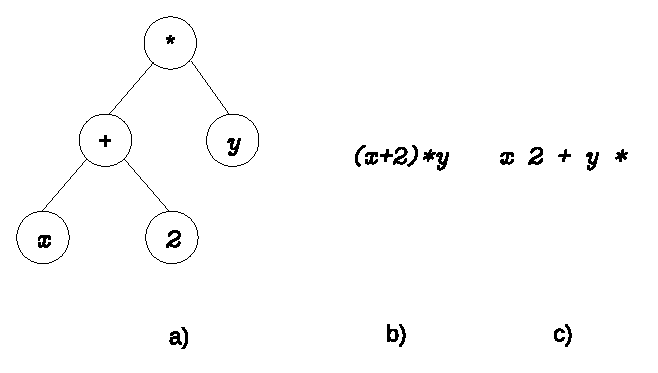
\includegraphics[scale=0.7]{images/02-02.eps}
  \caption{Various Concrete Syntaxes for Expression Language}
  \label{expression-concrete}
\end{figure}

Now we need to define the semantic domain for the semantics of expressions. We already hinted that this domain should be shaped like a set of some
data processing functions $\mathfrak{D}\to\mathfrak{D}$; however, we need to be more specific.

As we deal with arithmetic expressions it is rather natural to expect that the results of their evaluation are interger values, i.e. $\mathbb{Z}$ (as we agreed
earlier, we assume $\mathbb{Z}\subset\mathfrak{D}$); on the other hand, the value of an expression depends on the values of variables it contains. We can
encode these values as a \emph{state}~--- a function which maps variables to integer values:

\[
St : \mathscr{X} \to \mathbb{Z}
\]

There is nothing wrong with assuming $St\subset\mathfrak{D}$: as any expression can contain only a finite number of variables we are interested only in
states with finite domains which can be encoded, for example, as finite lists of pairs. Thus, finally, we have the following ``type'' for the semantics
of expressions:

\[
\sembr{\bullet}^\ph_\mathscr{E}:\mathscr{E}\to(St\to\mathbb{Z})
\]

\subsection{Denotational Semantics}

There are multiple ways to give the semantics for a language formally. Here we use so-called \emph{denotational} way in which it is immediately
specified what object from the semantic domain corresponds to a given language construct. For this concrete language denotational semantics
looks simple and natural; however, for more advanced languages more advanced mathematical apparatus would be required. It is also worth mentioning that,
as a rule, denotational semantics gives us a very abstract, high-level view on the behavior of programs, which may or may not be desirable from a
practical standpoint.


\begin{figure}[t]
\[
\begin{array}{rcl}
  \sembr{z}^\ph_\mathscr{E} & = & \sigma \mapsto z \\  
  \sembr{x}^\ph_\mathscr{E} & = & \sigma \mapsto \sigma\,x \\
  \sembr{e_1\otimes e_2}^\ph_\mathscr{E} & = & \sigma \mapsto \sembr{e_2}^\ph_\mathscr{E}\,\sigma\oplus\sembr{e_2}^\ph_\mathscr{E}\,\sigma
\end{array}
\]
\caption{Denotational Semantics of Expressions}
\label{se-denot}
\end{figure}


The denotational semantics for expressions is shown in Fig.~\ref{se-denot}.
We give here three equations, one for each syntactic form. In the right-hand side of each equation we immediately
give the object (a function from states to integers) which corresponds to the semantics of the expression in the
left-hand side. The notation $\star \mapsto \bullet$ is used to denote a function from $\star$ to $\bullet$; we refrain from
using the lambda notation since these functions are elements of the \emph{meta-language} (the language we use to describe the
semantics), not of the \emph{object} one (the language which semantics is being described).

In the first equation, when the expression is a natural number $z$, its semantics is a constant function, which for
any state $\sigma$ return just this number $z$.

When the expression in question is a variable $x$, its semantics is a function which, given a state $\sigma$, returns
the value this state assigns to this variable.

Finally, when the expression is a binary operator with two subexpressions $e_1$ and $e_2$, its semantics is a function which, given a state $\sigma$,
first calcalates the values of subexpressions $e_1$ and $e_2$ in the same state, and then combines them using a certain arithmetic operator $\oplus$.
The correspondence between $\otimes$ and $\oplus$ is described by the following table:

\begin{center}
\begin{tabular}{c|cl}
  $\otimes$     & $\oplus$ in \lama\\
  \hline
  $+$      & \lstinline|+|   \\
  $-$      & \lstinline|-|   \\
  $\times$ & \lstinline|*|   \\
  $/$      & \lstinline|/|   \\
  $\%$     & \lstinline|%|   \\
  $<$      & \lstinline|<|   \\
  $>$      & \lstinline|>|   \\
  $\le$    & \lstinline|<=|  \\
  $\ge$    & \lstinline|>=|  \\
  $=$      & \lstinline|=|   \\
  $\ne$    & \lstinline|!=|  \\
  $\wedge$ & \lstinline|&&|  \\
  $\vee$   & \lstinline/!!/ 
\end{tabular}
\end{center}

Here we use built-in \lama binary operators to specify the semantics of $\oplus$; this approach is good enough for now since our primary objective is
to implement a reference interpreter in \lama. Later, when we will deal with \texttt{x86} codegenerator we will refine the understanding of
these operators' semantics.

Note, while the symbols in the first and second columns look similar, they actually have different nature: the left ones are
elements of syntax while the right ones~--- conventional denotations for familiar arithmetic operators.
The last equation in Fig.~\ref{se-denot}, thus, is actually a generic one which denotes \emph{thirteen} concrete equations in which $\otimes$ and $\oplus$ are
substituted coherently according to the table given above.

We can make two important observations.

First, in given semantics there is a single rule for any ``kind'' of expression (variable, constant, binary operation), and for each rule its right part defines
semantic function unambiguously. Thus, for each expression $e$ and each state $\sigma$ there is \emph{at most} one
integer number $y$ such that

\[
  \sembr{e}^\ph_\mathscr{E}\,\sigma=x
\]

This to some extent justifies our desire for $\sembr{e}^\ph_\mathscr{E}$ to be a function from states to integers. Indeed, the
property we just established is \emph{functionality}. On the other hand, in the domain of semantics the same property has
another name: \emph{determinism}. Thus, the semantics in question is deterministic, meaning that evaluating any expression in a given state
delivers at most one value. Non-deterministic semantics, according to which there can be multiple such values, seemingly are not
compatible with our framework of semantic functions; nevertheless, such semantics exist, and there are ways to fix this incompatibility.
Further we will deal only with deterministic semantics. 

Another important property is \emph{compositionality}: the semantics of a construct is expressed in the terms of the semantics
of its proper subconstructs. Indeed, the first two equations are \emph{axioms}, meaning, that no expressions containing semantic
brackets ``$\sembr{\bullet}^\ph_\mathscr{E}$'' occur in the right-hand side; the third equation is not an axiom, but semantic
backets are applied only to proper subconstructs ($e_1$ and $e_2$) of the construct in question ($e$). Compositionality is
a distinctive property of denotational semantics; using other semantic description styles may or may not result in compositional
semantic specification.

When a semantic is compositional, a certain proof principle~--- \emph{structural induction}~--- can be used to establish
its properties. This technique is essentially a specific kind of mathematical induction applied to \emph{finite trees} rather than to
natural numbers. To prove by structural induction that some property holds for all trees one needs to prove, first, that this
property holds for all leaves (\emph{base of induction}); then, assuming that the property holds for all trees up to a certain
height (\emph{induction hypothesis}) one needs to prove that the property holds for all trees one level higher. We demonstrate
the application of this principle by the following example.

\subsection{Strictness}

We are going to prove the \emph{strictness} property of given semantics. It informally means that in order to calculate the
value for the whole expression one needs to calculate the values for all its subexpressions. First, we define the
following relation ``$\preceq$'' of one expression being a subexpression of another:

\[
\begin{array}{c}
  e^\prime \preceq e^\prime\otimes e \\
  e^\prime \preceq e\otimes e^\prime \\
  e\preceq e \\
  e^\prime\preceq e^{\prime\prime} \wedge e^{\prime\prime}\preceq e \Rightarrow e^\prime\preceq e
\end{array}  
\]

The first two lines define the \emph{immediate} subexpression relation while the last two~--- its \emph{reflexive-transitive}
closure. For example, for the expression $(x+2)*y$ all its subexpression are $(x+2)*y$, $x+2$, $y$, $x$, and $2$. 

\begin{lemma}[Strictness]
  For all $e$, $\sigma$ and $x$ if

  \[
  \sembr{e}^\ph_\mathscr{E}\,\sigma=x
  \]

  then for all $e^\prime\preceq e$ there exists $x^\prime$ such that

  \[
  \sembr{e^\prime}^\ph_\mathscr{E}\,\sigma=x^\prime
  \]
\end{lemma}
\begin{proof}
  For base case (variable and constant) the lemma holds vacuously since in both cases
  the only possible subexpressions are these expressions themselves.

  Assume the lemma holds for $e_1$ and $e_2$; we need to prove it holds for $e_1\otimes e_2$.
  By the definition of ``$\preceq$'' for any $e^\prime\preceq e_1\otimes e_2$ one of the
  following is true:

  \begin{enumerate}
  \item $e^\prime=e_1$, or
  \item $e^\prime=e_2$, or
  \item $e^\prime\preceq e_1$, or
  \item $e^\prime\preceq e_1$.
  \end{enumerate}

  By the condition of lemma we have $\sembr{e_1\otimes e_2}^\ph_\mathscr{E}\,\sigma=x$.
  By the definitiono of $\sembr{\bullet}^\ph_\mathscr{E}$ we have $\sembr{e_1}^\ph_\mathscr{E}\,\sigma\oplus\sembr{e_2}^\ph_\mathscr{E}\,\sigma=x$.
  By the definition of $\oplus$ there exist $x_1$ and $x_2$ such that

  \[
  \begin{array}{rcl}
    \sembr{e_1}^\ph_\mathscr{E}\,\sigma&=&x_1\\
    \sembr{e_2}^\ph_\mathscr{E}\,\sigma&=&x_2
  \end{array}
  \]

  If $e^\prime=e_1$ or $e^\prime=e_2$ then the lemma follows immediately.
  If $e^\prime\preceq e_1$ (or $e^\prime\preceq e_2$) the induction hypothesis can be applied as we just have proven that
  both $e_1$ and $e_2$ have some values being evaluated in the state $\sigma$.
\end{proof}

The strictness property, in particular, means that if variable $x$ is undefined in some state $\sigma$, then
any expression $e$, containing $x$, is also undefined in $\sigma$. Indeed, if $x$ occurs in $e$, then, naturally,
$x\preceq e$. If $\sigma\,x$ undefined but $\sembr{e}^\ph_\mathscr{E}\,\sigma$ not, this would contradict
the lemma we've just proven.

Now we can give precise answers to the questions asked in section~\ref{intro-semantics}.
The first question was if the expression \lstinline|0*(x/0)| evaluates to zero or undefined. Due to the strictness of our semantics it is undefined in
any state. Indeed

\[
\mbox{\lstinline|x/0|}\preceq \mbox{\lstinline|0*(x/0)|}
\]

and $\sembr{\mbox{\lstinline|x/0|}}^\ph_\mathscr{E}\,\sigma$ is
undefined for any state $\sigma$ since either \lstinline[mathescape=true]|$\sigma\,$x| is undefined or
\lstinline[mathescape=true]|$\sigma\,$x| is defined but \lstinline[mathescape=true]|$\sigma\,$x / 0| is
undefined due to the division by zero.

The second question was if \lstinline|1+x-x| is equivalent to \lstinline|1|. Again, by the strictness and the
fact that $\mbox{\lstinline|x|}\preceq\mbox{\lstinline|1+x-x|}$ we immediately have that for the \emph{empty state}
$\Lambda$, undefined for every variable $x$, $\sembr{1}^\ph_\mathscr{E}\,\Lambda=1$ but $\sembr{\mbox{\lstinline|1+x-x|}}^\ph_\mathscr{E}\,\Lambda$ is undefined.
Thus, these two expressions are not equivalent.

We stress that these answers are specific to the concrete semantics of expressions we described; for different semantics the answers can be different.

\section{Statements}

The other syntactic category of the straight line programs language is \emph{statements}. Its abstract syntax is given by the following
description:

\[
\renewcommand{\arraystretch}{1}
\begin{array}{rcl}  
  \mathscr S & = & \mbox{\lstinline|skip|} \\
             &   & \mathscr X \mbox{\lstinline|:=|} \;\mathscr E \\
             &   & \mbox{\lstinline|read (|} \mathscr X \mbox{\lstinline|)|} \\
             &   & \mbox{\lstinline|write (|} \mathscr E \mbox{\lstinline|)|} \\
             &   & \mathscr S \mbox{\lstinline|;|} \mathscr S
\end{array}
\]

Here $\mathscr E$ and $\mathscr X$ stand for the sets of expressions and variables, as in the previous section. The first four lines of abstract
syntax description define four \emph{primitive} statements: empty, assignment, input and output respectively. The fifth one makes it possible to
combine primitive statements info compositions. The order and subordination of composition counterparts strictly speaking is essential, thus

\begin{lstlisting}
   read (x); {y := x+4; write (y)}
\end{lstlisting}

and

\begin{lstlisting}
   {read (x); y := x+4}; write (y)
\end{lstlisting}

are different statements; we use here curved brackets ``\lstinline|{|'' and ``\lstinline|}|'' as elements of concrete syntax to reflect the
grouping of subtrees in abstract syntax tree.

\subsection{Big-Step Operational Semantics}

Our next step is to define the semantics for statements. We could use the denotational style as we did for expression, and it would work
just fine. However, as our language starts to evolve, the denotational style will be harder to use according to our intentions; in addition
studying yet another way for semantics' specification would make us more versatile.

The technique we are going to use is called \emph{big-step operational semantics}. Unlike denotational case, where a semantic object
is immediately given for each syntactic form, operational style involves the construction of intermediate \emph{evaluation relation}.
But first, as always, we need to specify the semantic domain for statements' semantics.

%  The form of this relation description is borrowed from mathematical logic's natural deduction approach.

From the syntactic form of statements it should be clear that we are dealing with a language with \emph{side effects}: there are read and
write statements, which, presumably, deal with some outer world, and assignment, which, presumably, changes the values of variables. From
the semantics of expressions we already know the notion of state, and we already know how to calculate the values of expressions in
given states. Thus, each statement modifies an \emph{enriched} state which consists of regular state and the outer world. We call this
enriched state \emph{configuration}. Thus, the set of all configuration is defined as

\[
\begin{array}{rcl}
  \mathscr C &=& St \times \mathscr W\\
  \mathscr W &=& \mathbb Z^* \times \mathbb Z^*
\end{array}
\]

where $\mathscr W$~--- a set of \emph{worlds}, each of which escapsulates some input-output stream pair. For
simplicity, we define the following operations for worlds:

\[
\begin{array}{rcl}
  \primi{read}{\inbr{xi,\,o}}    & = & \inbr{x,\,\inbr{i,\,o}}\\
  \primi{write}{x\,\inbr{i,\,o}} & = & \inbr{i,\,ox}\\
  \primi{out}{\inbr{i,\,o}}      & = & o
\end{array}
\]


Again, we define the semantics for this language 

\[
\sembr{\bullet}_{\mathscr S} : \mathscr S \mapsto \mathbb Z^* \to \mathbb Z^*
\]

with the semantic domain of partial functions from integer streams to integer streams. Again, we will
use \emph{big-step operational semantics}: we define a ternary relation ``$\Rightarrow_{\mathscr S}$''

\[
\Rightarrow_{\mathscr S} \subseteq \mathscr C \times \mathscr S \times \mathscr C
\]

where $\mathscr C$~--- a set of possible \emph{configurations} during a program execution.
We will write $c_1\xRightarrow{S}_{\mathscr S}c_2$ instead of $(c_1, S, c_2)\in\Rightarrow_{\mathscr S}$ and informally
interpret the former as ``the execution of a statement $S$ in a configuration $c_1$ completes with the configuration
$c_2$''.

The relation ``$\Rightarrow_{\mathscr S}$'' is defined by the following deductive system (see Fig.~\ref{bs_stmt}). The first
three rules are \emph{axioms} as they do not have any premises. Note, according to these rules sometimes a program
cannot do a step in a given configuration: a value of an expression can be undefined in a given state in rules
$\rulename{Assign}$ and $\rulename{Write}$, and there can be no input value in rule $\rulename{Read}$. This style of
a semantics description is called big-step operational semantics, since the results of a computation are
immediately observable at the right hand side of ``$\Rightarrow$'' and, thus, the computation is performed in
a single ``big'' step. And, again, this style of a semantic description can be used to easily implement a
reference interpreter.

With the relation ``$\Rightarrow_{\mathscr S}$'' defined we can abbreviate the ``surface'' semantics for the language of statements:

\setarrow{\xRightarrow}
\setsubarrow{_{\mathscr S}}
\[
\trule{\trans{\inbr{\Lambda,\,\inbr{i,\,\epsilon}}}{S}{\inbr{\sigma,\,\omega}}}
      {\sembr{S}_{\mathscr S}i=\primi{out}{\omega}}
\]


\begin{figure}[t]
\arraycolsep=10pt
\[\trans{c}{\llang{skip}}{c}\ruleno{Skip}\]
\[\trans{\inbr{\sigma,\, \omega}}{\llang{x := $\;\;e$}}{\inbr{\sigma\,[x\gets\sembr{e}_{\mathscr E}\;\sigma],\,\omega}}\ruleno{Assign}\]
\[\trule{\inbr{z,\,\omega^\prime}=\primi{read}{\omega}}
        {\trans{\inbr{\sigma,\, \omega}}{\llang{read ($x$)}}{\inbr{\sigma\,[x\gets z],\,\omega^\prime}}}\ruleno{Read}\]
\[\trans{\inbr{\sigma,\, \omega}}{\llang{write ($e$)}}{\inbr{\sigma,\, \primi{write}{(\sembr{e}_{\mathscr E}\;\sigma)\, \omega}}}\ruleno{Write}\]
\[\trule{\begin{array}{cc}
            \trans{c_1}{S_1}{c^\prime} & \trans{c^\prime}{S_2}{c_2}
         \end{array}}
        {\trans{c_1}{S_1\llang{;}S_2}{c_2}}\ruleno{Seq}\]
\caption{Big-step operational semantics for statements}
\label{bs_stmt}
\end{figure}






